% Created by tikzDevice version 0.10.1 on 2016-07-24 20:43:58
% !TEX encoding = UTF-8 Unicode
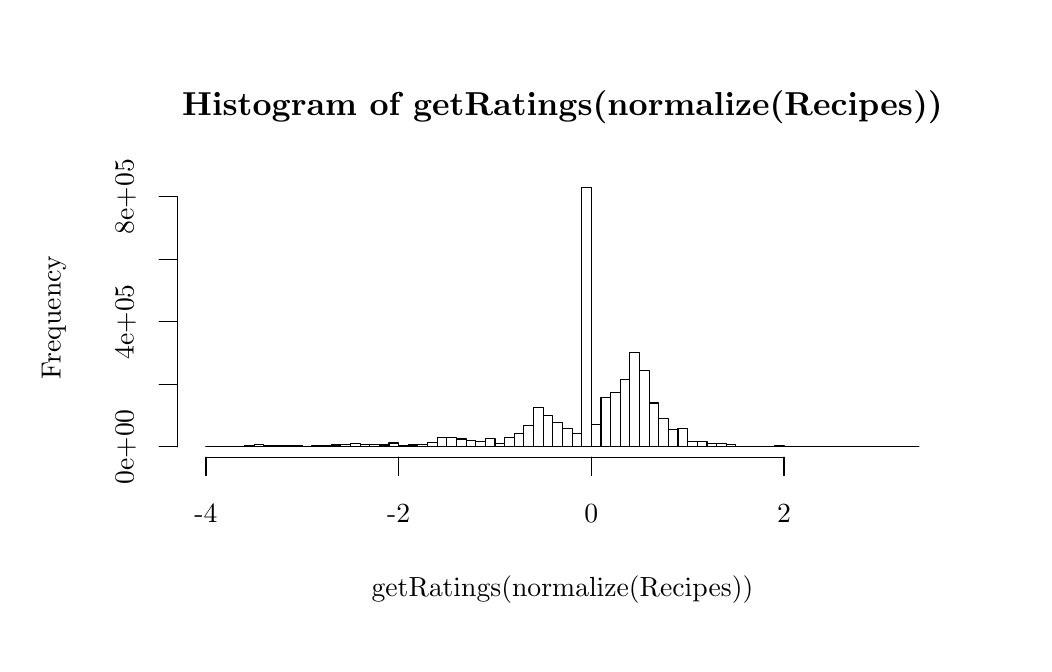
\begin{tikzpicture}[x=1pt,y=1pt]
\definecolor{fillColor}{RGB}{255,255,255}
\path[use as bounding box,fill=fillColor,fill opacity=0.00] (0,0) rectangle (360.07,222.54);
\begin{scope}
\path[clip] (  0.00,  0.00) rectangle (360.07,222.54);
\definecolor{drawColor}{RGB}{0,0,0}

\node[text=drawColor,anchor=base,inner sep=0pt, outer sep=0pt, scale=  1.20] at (193.24,190.95) {\bfseries Histogram of getRatings(normalize(Recipes))};

\node[text=drawColor,anchor=base,inner sep=0pt, outer sep=0pt, scale=  1.00] at (193.24, 17.16) {getRatings(normalize(Recipes))};

\node[text=drawColor,rotate= 90.00,anchor=base,inner sep=0pt, outer sep=0pt, scale=  1.00] at ( 11.88,117.87) {Frequency};
\end{scope}
\begin{scope}
\path[clip] (  0.00,  0.00) rectangle (360.07,222.54);
\definecolor{drawColor}{RGB}{0,0,0}

\path[draw=drawColor,line width= 0.4pt,line join=round,line cap=round] ( 64.42, 67.32) -- (273.31, 67.32);

\path[draw=drawColor,line width= 0.4pt,line join=round,line cap=round] ( 64.42, 67.32) -- ( 64.42, 60.72);

\path[draw=drawColor,line width= 0.4pt,line join=round,line cap=round] (134.05, 67.32) -- (134.05, 60.72);

\path[draw=drawColor,line width= 0.4pt,line join=round,line cap=round] (203.68, 67.32) -- (203.68, 60.72);

\path[draw=drawColor,line width= 0.4pt,line join=round,line cap=round] (273.31, 67.32) -- (273.31, 60.72);

\node[text=drawColor,anchor=base,inner sep=0pt, outer sep=0pt, scale=  1.00] at ( 64.42, 43.56) {-4};

\node[text=drawColor,anchor=base,inner sep=0pt, outer sep=0pt, scale=  1.00] at (134.05, 43.56) {-2};

\node[text=drawColor,anchor=base,inner sep=0pt, outer sep=0pt, scale=  1.00] at (203.68, 43.56) {0};

\node[text=drawColor,anchor=base,inner sep=0pt, outer sep=0pt, scale=  1.00] at (273.31, 43.56) {2};

\path[draw=drawColor,line width= 0.4pt,line join=round,line cap=round] ( 54.12, 71.06) -- ( 54.12,161.42);

\path[draw=drawColor,line width= 0.4pt,line join=round,line cap=round] ( 54.12, 71.06) -- ( 47.52, 71.06);

\path[draw=drawColor,line width= 0.4pt,line join=round,line cap=round] ( 54.12, 93.65) -- ( 47.52, 93.65);

\path[draw=drawColor,line width= 0.4pt,line join=round,line cap=round] ( 54.12,116.24) -- ( 47.52,116.24);

\path[draw=drawColor,line width= 0.4pt,line join=round,line cap=round] ( 54.12,138.83) -- ( 47.52,138.83);

\path[draw=drawColor,line width= 0.4pt,line join=round,line cap=round] ( 54.12,161.42) -- ( 47.52,161.42);

\node[text=drawColor,rotate= 90.00,anchor=base,inner sep=0pt, outer sep=0pt, scale=  1.00] at ( 38.28, 71.06) {0e+00};

\node[text=drawColor,rotate= 90.00,anchor=base,inner sep=0pt, outer sep=0pt, scale=  1.00] at ( 38.28,116.24) {4e+05};

\node[text=drawColor,rotate= 90.00,anchor=base,inner sep=0pt, outer sep=0pt, scale=  1.00] at ( 38.28,161.42) {8e+05};
\end{scope}
\begin{scope}
\path[clip] ( 54.12, 67.32) rectangle (332.35,168.42);
\definecolor{drawColor}{RGB}{0,0,0}

\path[draw=drawColor,line width= 0.4pt,line join=round,line cap=round] ( 64.42, 71.06) rectangle ( 67.91, 71.07);

\path[draw=drawColor,line width= 0.4pt,line join=round,line cap=round] ( 67.91, 71.06) rectangle ( 71.39, 71.08);

\path[draw=drawColor,line width= 0.4pt,line join=round,line cap=round] ( 71.39, 71.06) rectangle ( 74.87, 71.13);

\path[draw=drawColor,line width= 0.4pt,line join=round,line cap=round] ( 74.87, 71.06) rectangle ( 78.35, 71.26);

\path[draw=drawColor,line width= 0.4pt,line join=round,line cap=round] ( 78.35, 71.06) rectangle ( 81.83, 71.64);

\path[draw=drawColor,line width= 0.4pt,line join=round,line cap=round] ( 81.83, 71.06) rectangle ( 85.31, 71.87);

\path[draw=drawColor,line width= 0.4pt,line join=round,line cap=round] ( 85.31, 71.06) rectangle ( 88.79, 71.57);

\path[draw=drawColor,line width= 0.4pt,line join=round,line cap=round] ( 88.79, 71.06) rectangle ( 92.28, 71.51);

\path[draw=drawColor,line width= 0.4pt,line join=round,line cap=round] ( 92.28, 71.06) rectangle ( 95.76, 71.43);

\path[draw=drawColor,line width= 0.4pt,line join=round,line cap=round] ( 95.76, 71.06) rectangle ( 99.24, 71.57);

\path[draw=drawColor,line width= 0.4pt,line join=round,line cap=round] ( 99.24, 71.06) rectangle (102.72, 71.26);

\path[draw=drawColor,line width= 0.4pt,line join=round,line cap=round] (102.72, 71.06) rectangle (106.20, 71.38);

\path[draw=drawColor,line width= 0.4pt,line join=round,line cap=round] (106.20, 71.06) rectangle (109.68, 71.42);

\path[draw=drawColor,line width= 0.4pt,line join=round,line cap=round] (109.68, 71.06) rectangle (113.16, 71.75);

\path[draw=drawColor,line width= 0.4pt,line join=round,line cap=round] (113.16, 71.06) rectangle (116.65, 72.07);

\path[draw=drawColor,line width= 0.4pt,line join=round,line cap=round] (116.65, 71.06) rectangle (120.13, 72.32);

\path[draw=drawColor,line width= 0.4pt,line join=round,line cap=round] (120.13, 71.06) rectangle (123.61, 72.00);

\path[draw=drawColor,line width= 0.4pt,line join=round,line cap=round] (123.61, 71.06) rectangle (127.09, 71.97);

\path[draw=drawColor,line width= 0.4pt,line join=round,line cap=round] (127.09, 71.06) rectangle (130.57, 71.73);

\path[draw=drawColor,line width= 0.4pt,line join=round,line cap=round] (130.57, 71.06) rectangle (134.05, 72.48);

\path[draw=drawColor,line width= 0.4pt,line join=round,line cap=round] (134.05, 71.06) rectangle (137.53, 71.43);

\path[draw=drawColor,line width= 0.4pt,line join=round,line cap=round] (137.53, 71.06) rectangle (141.01, 71.73);

\path[draw=drawColor,line width= 0.4pt,line join=round,line cap=round] (141.01, 71.06) rectangle (144.50, 72.00);

\path[draw=drawColor,line width= 0.4pt,line join=round,line cap=round] (144.50, 71.06) rectangle (147.98, 72.71);

\path[draw=drawColor,line width= 0.4pt,line join=round,line cap=round] (147.98, 71.06) rectangle (151.46, 74.39);

\path[draw=drawColor,line width= 0.4pt,line join=round,line cap=round] (151.46, 71.06) rectangle (154.94, 74.31);

\path[draw=drawColor,line width= 0.4pt,line join=round,line cap=round] (154.94, 71.06) rectangle (158.42, 73.89);

\path[draw=drawColor,line width= 0.4pt,line join=round,line cap=round] (158.42, 71.06) rectangle (161.90, 73.41);

\path[draw=drawColor,line width= 0.4pt,line join=round,line cap=round] (161.90, 71.06) rectangle (165.38, 72.87);

\path[draw=drawColor,line width= 0.4pt,line join=round,line cap=round] (165.38, 71.06) rectangle (168.87, 74.07);

\path[draw=drawColor,line width= 0.4pt,line join=round,line cap=round] (168.87, 71.06) rectangle (172.35, 72.43);

\path[draw=drawColor,line width= 0.4pt,line join=round,line cap=round] (172.35, 71.06) rectangle (175.83, 74.53);

\path[draw=drawColor,line width= 0.4pt,line join=round,line cap=round] (175.83, 71.06) rectangle (179.31, 75.81);

\path[draw=drawColor,line width= 0.4pt,line join=round,line cap=round] (179.31, 71.06) rectangle (182.79, 78.92);

\path[draw=drawColor,line width= 0.4pt,line join=round,line cap=round] (182.79, 71.06) rectangle (186.27, 85.27);

\path[draw=drawColor,line width= 0.4pt,line join=round,line cap=round] (186.27, 71.06) rectangle (189.75, 82.39);

\path[draw=drawColor,line width= 0.4pt,line join=round,line cap=round] (189.75, 71.06) rectangle (193.24, 80.02);

\path[draw=drawColor,line width= 0.4pt,line join=round,line cap=round] (193.24, 71.06) rectangle (196.72, 77.83);

\path[draw=drawColor,line width= 0.4pt,line join=round,line cap=round] (196.72, 71.06) rectangle (200.20, 75.83);

\path[draw=drawColor,line width= 0.4pt,line join=round,line cap=round] (200.20, 71.06) rectangle (203.68,164.68);

\path[draw=drawColor,line width= 0.4pt,line join=round,line cap=round] (203.68, 71.06) rectangle (207.16, 79.01);

\path[draw=drawColor,line width= 0.4pt,line join=round,line cap=round] (207.16, 71.06) rectangle (210.64, 88.97);

\path[draw=drawColor,line width= 0.4pt,line join=round,line cap=round] (210.64, 71.06) rectangle (214.12, 90.73);

\path[draw=drawColor,line width= 0.4pt,line join=round,line cap=round] (214.12, 71.06) rectangle (217.60, 95.34);

\path[draw=drawColor,line width= 0.4pt,line join=round,line cap=round] (217.60, 71.06) rectangle (221.09,105.02);

\path[draw=drawColor,line width= 0.4pt,line join=round,line cap=round] (221.09, 71.06) rectangle (224.57, 98.79);

\path[draw=drawColor,line width= 0.4pt,line join=round,line cap=round] (224.57, 71.06) rectangle (228.05, 86.93);

\path[draw=drawColor,line width= 0.4pt,line join=round,line cap=round] (228.05, 71.06) rectangle (231.53, 81.39);

\path[draw=drawColor,line width= 0.4pt,line join=round,line cap=round] (231.53, 71.06) rectangle (235.01, 77.22);

\path[draw=drawColor,line width= 0.4pt,line join=round,line cap=round] (235.01, 71.06) rectangle (238.49, 77.73);

\path[draw=drawColor,line width= 0.4pt,line join=round,line cap=round] (238.49, 71.06) rectangle (241.97, 72.97);

\path[draw=drawColor,line width= 0.4pt,line join=round,line cap=round] (241.97, 71.06) rectangle (245.46, 72.96);

\path[draw=drawColor,line width= 0.4pt,line join=round,line cap=round] (245.46, 71.06) rectangle (248.94, 72.12);

\path[draw=drawColor,line width= 0.4pt,line join=round,line cap=round] (248.94, 71.06) rectangle (252.42, 72.28);

\path[draw=drawColor,line width= 0.4pt,line join=round,line cap=round] (252.42, 71.06) rectangle (255.90, 72.05);

\path[draw=drawColor,line width= 0.4pt,line join=round,line cap=round] (255.90, 71.06) rectangle (259.38, 71.32);

\path[draw=drawColor,line width= 0.4pt,line join=round,line cap=round] (259.38, 71.06) rectangle (262.86, 71.34);

\path[draw=drawColor,line width= 0.4pt,line join=round,line cap=round] (262.86, 71.06) rectangle (266.34, 71.24);

\path[draw=drawColor,line width= 0.4pt,line join=round,line cap=round] (266.34, 71.06) rectangle (269.83, 71.13);

\path[draw=drawColor,line width= 0.4pt,line join=round,line cap=round] (269.83, 71.06) rectangle (273.31, 71.61);

\path[draw=drawColor,line width= 0.4pt,line join=round,line cap=round] (273.31, 71.06) rectangle (276.79, 71.07);

\path[draw=drawColor,line width= 0.4pt,line join=round,line cap=round] (276.79, 71.06) rectangle (280.27, 71.09);

\path[draw=drawColor,line width= 0.4pt,line join=round,line cap=round] (280.27, 71.06) rectangle (283.75, 71.08);

\path[draw=drawColor,line width= 0.4pt,line join=round,line cap=round] (283.75, 71.06) rectangle (287.23, 71.10);

\path[draw=drawColor,line width= 0.4pt,line join=round,line cap=round] (287.23, 71.06) rectangle (290.71, 71.07);

\path[draw=drawColor,line width= 0.4pt,line join=round,line cap=round] (290.71, 71.06) rectangle (294.20, 71.07);

\path[draw=drawColor,line width= 0.4pt,line join=round,line cap=round] (294.20, 71.06) rectangle (297.68, 71.08);

\path[draw=drawColor,line width= 0.4pt,line join=round,line cap=round] (297.68, 71.06) rectangle (301.16, 71.07);

\path[draw=drawColor,line width= 0.4pt,line join=round,line cap=round] (301.16, 71.06) rectangle (304.64, 71.07);

\path[draw=drawColor,line width= 0.4pt,line join=round,line cap=round] (304.64, 71.06) rectangle (308.12, 71.07);

\path[draw=drawColor,line width= 0.4pt,line join=round,line cap=round] (308.12, 71.06) rectangle (311.60, 71.06);

\path[draw=drawColor,line width= 0.4pt,line join=round,line cap=round] (311.60, 71.06) rectangle (315.08, 71.06);

\path[draw=drawColor,line width= 0.4pt,line join=round,line cap=round] (315.08, 71.06) rectangle (318.56, 71.06);

\path[draw=drawColor,line width= 0.4pt,line join=round,line cap=round] (318.56, 71.06) rectangle (322.05, 71.06);
\end{scope}
\end{tikzpicture}
